\chapter{System Development}
\label{chp:project}

\section{System Architecture Design}
The design of the system was a crucial part of my internship, consuming approximately 20\% of the total hours dedicated to the project. It was crafted to meet the specific requirements of the business while also taking into account the current context and future needs of the company. UNOX, having collaborated with \ac{AWS} since 2019, leverages innovative \ac{AWS} technologies to maintain a competitive edge. For this project, we were guided by an \ac{AWS} Solution Architect and an Enterprise Account Manager, who played a pivotal role in helping us build a cutting-edge system that adheres to \ac{AWS}'s Well-Architected Framework principles, ensuring Operational Excellence, Reliability, Performance Efficiency, Security, Cost Optimization, and Sustainability.

The \ac{AWS} Solution Architect, in particular, provided detailed comparisons of the various \ac{AWS} technologies available, enabling key decision-makers such as myself, the team leader, and the company's CTO to gain a comprehensive understanding of the potential architectures we could build. During the early stages of my internship, we held recurring meetings to explore potential solutions that best aligned with our specific requirements and the nature of UNOX's business operations. These discussions helped us identify the ideal path forward, though the initial solutions inevitably evolved as we encountered and addressed practical challenges during the system's development.

A core aspect of the system design was to ensure a clear separation between the storage layer and the business analytics layer, effectively decoupling data producers (such as operational systems) from data consumers (like reporting and predictive analytics systems). This separation was essential to facilitate data science activities, where a data lake provides a convenient storage layer for experimental data, supporting both the input and output of data analysis and machine learning tasks. The architecture also needed to support autonomous creation and use of data, without the need for coordination between programs or analysts, while at the same time enabling the sharing and re-use of massive datasets through a distributed computational framework.

\subsection{Data Lake vs. Data Warehouse vs. Data Lakehouse}
The initial idea for this project was to implement a data lake, a more innovative and flexible approach compared to traditional data warehouses. While both are used for storing large volumes of data, they serve different purposes and have distinct architectural characteristics.

Traditionally, a \textbf{data warehouse} is optimized for structured data, meaning data is cleaned, organized, and stored in a predefined schema, making it ideal for business reporting and analytics. However, data warehouses typically involve high setup and maintenance costs, and they require significant preprocessing to ensure data consistency before it can be used for analysis. Hence, they suffer from limited flexibility for advanced analytics, including machine learning tasks.

A \textbf{data lake}, on the other hand, offers a more flexible storage solution. It is capable of storing vast amounts of both structured and unstructured data in its raw form, allowing for greater adaptability. This means that data lakes are not bound by rigid schemas and can accommodate data from diverse sources without the need for heavy preprocessing. Data lakes are particularly suitable for data science, machine learning, and exploratory analysis, as they allow analysts and data scientists to directly interact with raw data, creating an environment where experimentation can thrive. A detailed analysis of the differences between data warehouses and data lakes is given in Table \ref{tab:dataw} \cite{nambiar2022overview}.

\begin{table}[h!]
\centering
\begin{tabular}{|p{2.5cm}|p{6.25cm}|p{6.25cm}|}
\hline
\textbf{Parameters}        & \textbf{Data Warehouse}                                      & \textbf{Data Lake}  \\ \hline
\textbf{Data}              & Focuses only on business processes                           & Stores everything   \\ \hline
\textbf{Processing}        & Highly processed data                                        & Mainly unprocessed data                                     \\ \hline
\textbf{Type of Data}      & Mostly in tabular form and structured                        & Can be unstructured, semi-structured, or structured  \\ \hline
\textbf{Task}              & Optimized for data retrieval                                 & Share data stewardship  \\ \hline
\textbf{Agility}           & Less agile, has a fixed configuration                        & Highly agile, can be configured and reconfigured as needed \\ \hline
\textbf{Users}             & Widely used by business professionals and business analysts  & Used by data scientists, data developers, and business analysts  \\ \hline
\textbf{Storage}           & Expensive storage for fast response times                    & Designed for low-cost storage                                       \\ \hline
\textbf{Security}          & Allows better control of the data                            & Offers less control  \\ \hline
\textbf{Schema}            & Schema on writing (predefined schemas)                       & Schema on reading (no predefined schemas)                           \\ \hline
\textbf{Data Processing}   & Time-consuming to introduce new content                      & Helps with fast ingestion of new data                               \\ \hline
\textbf{Data Granularity}  & Data at the summary or aggregated level of detail            & Data at a low level of detail or granularity                        \\ \hline
\textbf{Tools}             & Mostly commercial tools                                      & Can use open-source tools such as Hadoop or MapReduce             \\ \hline
\end{tabular}
\caption{Comparison between Data Warehouse and Data Lake}
\label{tab:dataw}
\end{table}

For this project, the data lake was selected because it enables autonomous data handling, and data producers do not need to coordinate directly with consumers. It also provides a shared storage framework, which facilitates collaboration between teams and allows for the re-use of large datasets without duplication or complex integration.

However, while data lakes excel in flexibility, they can sometimes suffer from challenges related to data governance, data quality, performance, and metadata management. As a result, organizations have adopted a two-tier architecture: storing data in lakes and then moving curated data to warehouses for structured analytics.
The two-tier model (data lakes + data warehouses) introduces new complexities, including reliability and cost issues. Indeed, maintaining consistency between the lake and warehouse is complex and storing data in two places and running ETL processes increase costs.

This is where a more modern architecture, the \textbf{Data Lakehouse} \cite{armbrust2021lakehouse}, promoted by Databricks\footnote{\url{https://www.databricks.com/}}, a cloud platform built on Apache Spark that enables unified data analytics, machine learning, and big data processing, comes into play.

The lakehouse architecture combines the best features of both data lakes and data warehouses. It retains the ability of a data lake to store raw and semi-structured data while incorporating some of the data management and performance optimization features of a data warehouse. This hybrid approach allows for real-time analytics and \ac{ACID} transactions on large datasets by adding structured layers of metadata to the raw data.
In fact, the system developed in this project can be interpreted as a data lakehouse. Although it functions primarily as a data lake, we have integrated several layers that provide pre-aggregated tables in Parquet or Iceberg formats, which are directly usable for advanced analysis. These formats not only offer significant performance benefits through better compression and faster query times but also enable \ac{ACID} operations. This structured approach allows us to maximize the system's potential for advanced business intelligence while maintaining the flexibility and scalability inherent in a data lake.

\subsection{The whole system}

\begin{figure}[H]
    \centering
    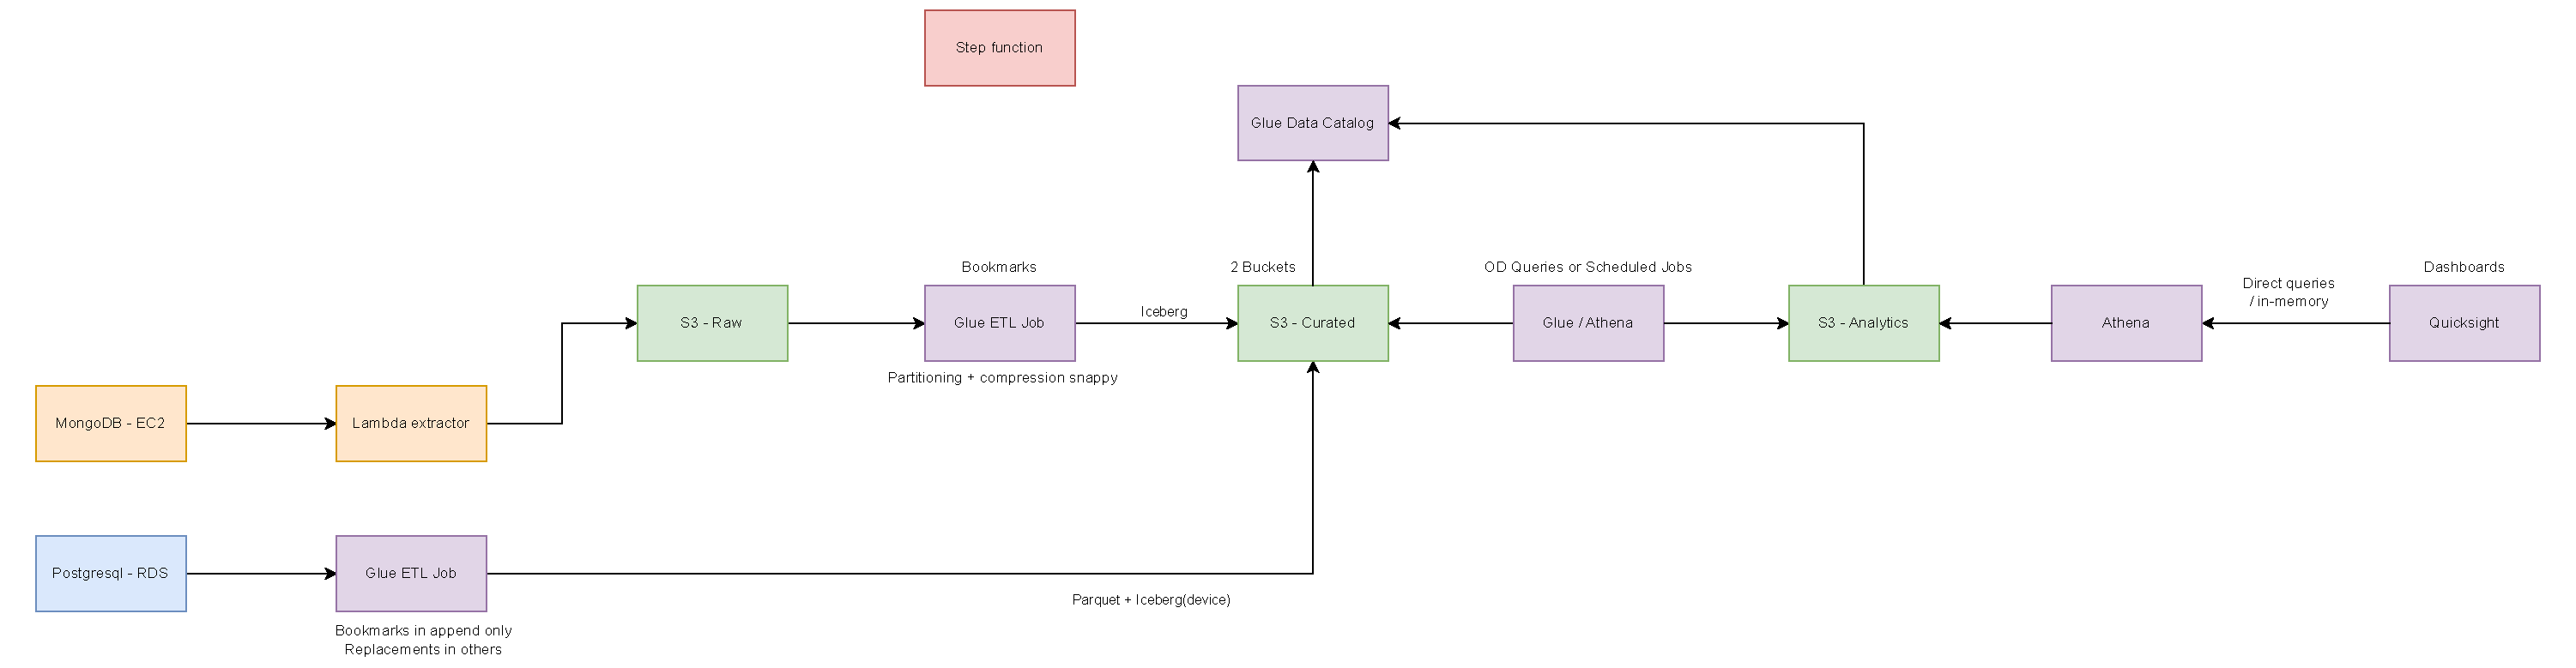
\includegraphics[width=1\textwidth]{res/unox-datalake-v2.pdf}
    \caption{The Whole System}
    \label{fig:wholesystem}
\end{figure}


\section{Data Sources}

\section{Data Ingestion}

\section{Data Integration}

\section{Data Cataloguing}

\section{Direct Queries}

\section{Report creation}

\section{Orchestration and Scheduling}